
%%%%%%%%%%%%%%%%%%%%%%%%%%%%%%%%%%%%%%%%%%
\begin{frame}
    \frametitle{}
    \begin{center}
    { {\huge 第四讲、态叠加原理}}
    \end{center}    
\end{frame}
%%%%%%%%%%%%%%%%%%%%%%%%%%%%%%%%%%%%%


\section{前情回顾}

\begin{frame}
    \frametitle{前情回顾}
    \begin{itemize}
        \item 波粒二象性
        \item 波函数假说
        \item 波函数的统计解释
    \end{itemize}
\end{frame}  

\section{经典叠加}

\begin{frame}
    \frametitle{经典叠加}
    \begin{center}
        \includegraphics[width=0.5\textwidth]{figs/sup-2.png} \\
    \end{center} 
    依据统计解释,振幅的概率幅\\
    \begin{itemize}
        \item 小球双缝实验,$P'=P_1+P_2 $, 是概率叠加。
        \item 经典叠加是概率叠加!
    \end{itemize}
\end{frame} 

\section{态叠加原理}

\begin{frame}
    \frametitle{态叠加}
    \begin{center}
        \includegraphics[width=0.5\textwidth]{figs/sup-3.png} \\
    \end{center} 
    依据统计解释,振幅的概率幅\\
    \begin{itemize}
        \item 电子双缝实验,$P\neq P_1+P_2 $,不是概率叠加!
        \item 波恩认为服从波函数(态)叠加
        $$ \psi =\psi_1+\psi_2$$
    \end{itemize}
\end{frame} 


\begin{frame} [allowframebreaks=]
    Explanation of the two-slit experiment.\\
    \begin{itemize}
        \item Lets $\psi_1$ describe the state of the electron run across slit-1 and $\psi_2$ for slit-2. \\
        \item when both of them are opened, the electron locates the superposition 
            \[ \Psi=c_1 \psi_1+ c_2\psi_2 \]
        \item the possiblity of electron reaches each point of screen 
    \begin{equation*}
        \begin{split}
            \omega &=|\Psi|^2 \\
            &= (c_1 \psi_1+ c_2\psi_2)^* (c_1 \psi_1+ c_2\psi_2) \\
            &=(\psi_1^*+\psi_2^*)(\psi_1+\psi_2) \\ 
            & = |c_1|^2 |\psi_1|^2 + |c_2|^2 |\psi_2|^2  + [c_1 c_2 ^* \psi_1 \psi_2 ^* + c_1 ^* c_2 \psi_1 ^* \psi_2] \\
        \end{split} 
    \end{equation*}
        \item interference pattern comes from  
     \[[c_1 C_c ^* \psi_1 \psi_2 ^* + c_1 ^* c_2 \psi_1 ^* \psi_2] \]
    \end{itemize}
    \begin{itemize}
        \item 概率计算发现,存在干涉项(后两项),产生干涉条纹。
        \item 电子如果只过一个缝,则$\psi_1$ 或$\psi_2$为零,干涉项为零,没有干涉条纹!
        \item 干涉条纹正是源于电子同时过两个缝, 即电子处于叠加态。
    \end{itemize}
    基于此,波恩提出了态叠加原理
\end{frame}

\begin{frame}
    \frametitle{态叠加原理}
    \begin{tcolorbox1}{Superposition principle of states}
    Born also proposed that: \\
    if $\psi_1$ and $\psi_2$ are the possible states of the system,
    their linear superposition \[ \Psi=c_1 \psi_1+ c_2\psi_2 \]
    is also the possible state of the system.\\
    if the system locates at the superposition $\Psi$, the possiblity of observating the system at $\psi_1$ is $|c_1|^2$, and at $\psi_2$ is $|c_2|^2$ \\
    \[\sum_i |c_i|^2 =1\]
    \end{tcolorbox1}
\end{frame}

\begin{frame}
    \frametitle{}
    \begin{tcolorbox}[colback=yellow!10,colframe=red!75!black,title=态叠加原理]
    如果 $\psi_1$ 、 $\psi_2$、 $\cdots$、$\psi_N$ 是粒子可能的态,那么它们的线性叠加
        $$ \Psi=c_1 \psi_1+ c_2\psi_2+\cdots+c_N\psi_N $$
    也是粒子可能的态(称为叠加态)\\   
    如果粒子处于叠加态 $\Psi=\sum\limits_{i=1}^N c_i \psi_i$,  
    那么测量粒子处在 $\psi_i$ 态的概率为 $\|c_i\|^2$\\ 
    并且  $$\sum_{i=1}^{N} |c_i|^2 =1$$
    \end{tcolorbox}
\end{frame}

\begin{frame}
    \frametitle{实验升级}
    \begin{center}
        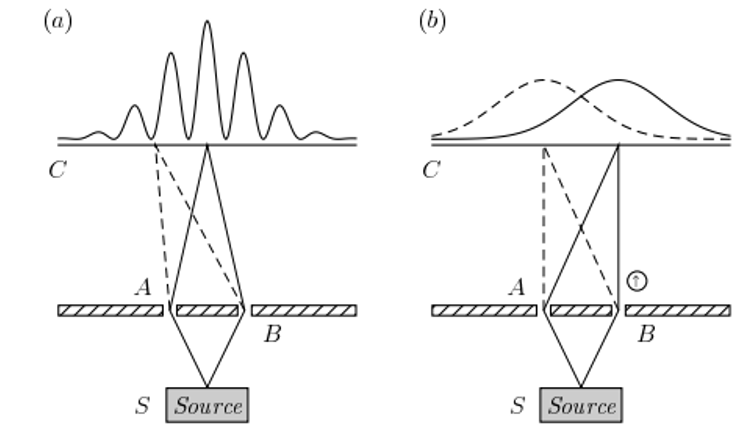
\includegraphics[width=0.5\textwidth]{figs/sup-4.png} \\
    \end{center} 
    \begin{itemize}
        \item 目标:想观测到电子是如何同时过两个缝的
        \item 结果:1)只能测到电子要么过第一缝,要么过第二缝。\\
        2)探测器越灵敏,干涉条纹越模糊,\\
        3) 当探测器能长时间地保持几乎可以完全判断电子过哪条缝时,干涉条纹消失!如图(b)所示
    \end{itemize}
\end{frame}

\begin{frame} [allowframebreaks=]
    \frametitle{结果分析}
    \begin{enumerate}
        \item 测量目的与结果\\
        \begin{itemize}
            \item 当我们“挖出”A和B两条狭缝时,“设计”了一个想要观察“电子的波动性”的设备,也就是电子已经预先被我们设定为“波”,因此我们观测到波动性(干涉条纹)
            \item 当我们装上侦测器时,整个实验被我们“设计”成观察电子的“粒子性”,因为想要知道电子到底是由A还是B穿过时,就必须先具备确定的“位置”的概念,因此我们观察到粒子性(干涉条纹消失)
        \end{itemize}
        \item 测量导致状态发生改变 \\
        \begin{itemize}
            \item 探测前,电子处于叠加态($ \psi =\psi_1+\psi_2$)
            \item 探测时,电子状态改变,被迫从叠加态变变为确定态 ($\psi_1$ or $\psi_2$),称为波函数坍塌
            \item 探测后,电子处于某一单态,不能干涉。
            \item 探测器不灵敏,有部分没有被探测到的电子依然处于叠加态, 干涉条纹模糊。
            \item 探测器灵敏,全部电子被探测,没有电子处于叠加态, 干涉条纹消失。
        \end{itemize}
        \item 测量结果互补(互补性原理)\\
        \begin{itemize}
            \item 波动性和粒子性是两种不同的属性,
            \item 不能因为测得粒子性就否定波动性,反之亦然。
            \item 测量结果就算相互矛盾,也要接受,它们互补地揭示物体的本质。
        \end{itemize}
        \item 结论
        \begin{itemize}
            \item 电子具有波粒二象性,总是处于叠加态
            \item 不被测量,则依然保持在叠加态
            \item 测量导致确定态出来,但结果是随机的。
            \item 测得某个确定态,不能说明电子原本就处于这个态
        \end{itemize}
    \end{enumerate}
\end{frame}

\section{Which Way?}

\begin{frame}
    \frametitle{Which Way?}
    The probabilistic interpretation was controversial from the beginning of of quantum mechanics
    \begin{itemize}
        \item De Broglie : Pilot waves
        \item Schr$\ddot{o}$dinger: Schr$\ddot{o}$dinger's cat
        \item Einstein: EPR paradox
        \item Wheeler's delayed choice experiment
        \item Quantum eraser experiment
        \item $\cdots \cdots$
    \end{itemize}
\end{frame}

\begin{frame}
    \frametitle{薛定谔的猫}
    \begin{center}
        \includegraphics[width=0.8\textwidth]{figs/cat.jpeg} \\
    \end{center} 
\end{frame}

\begin{frame}
    \frametitle{EPR佯谬}
    \begin{center}
        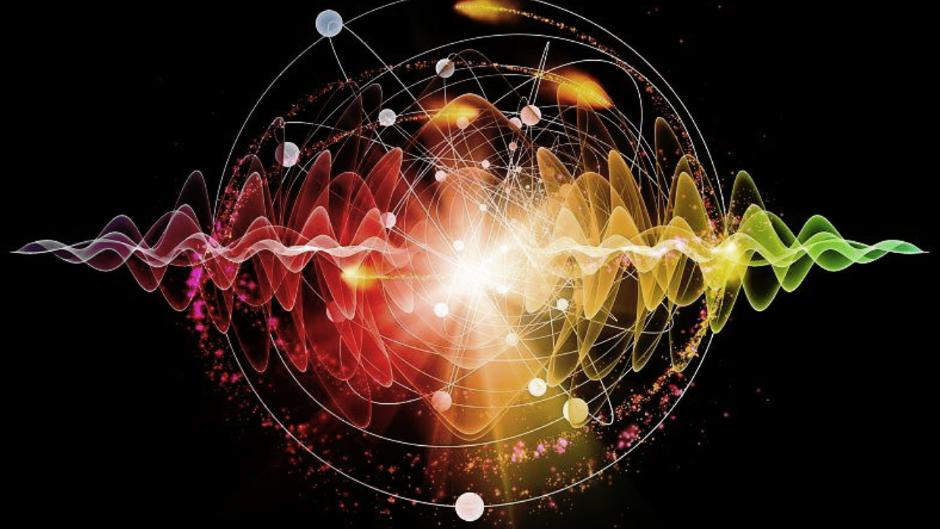
\includegraphics[width=1.0\textwidth]{figs/EPR.jpeg} \\
    \end{center} 
\end{frame}

\begin{frame}
    \frametitle{贝尔不等式}
    \begin{center}
        \includegraphics[width=1.0\textwidth]{figs/bell.png} \\
    \end{center} 
\end{frame}

\begin{frame}
    \frametitle{惠勒延迟选择实验}
    \begin{center}
        \includegraphics[width=0.8\textwidth]{figs/choose.png} \\
    \end{center} 
\end{frame}

\begin{frame}
    \frametitle{量子擦除实验}
    \begin{center}
        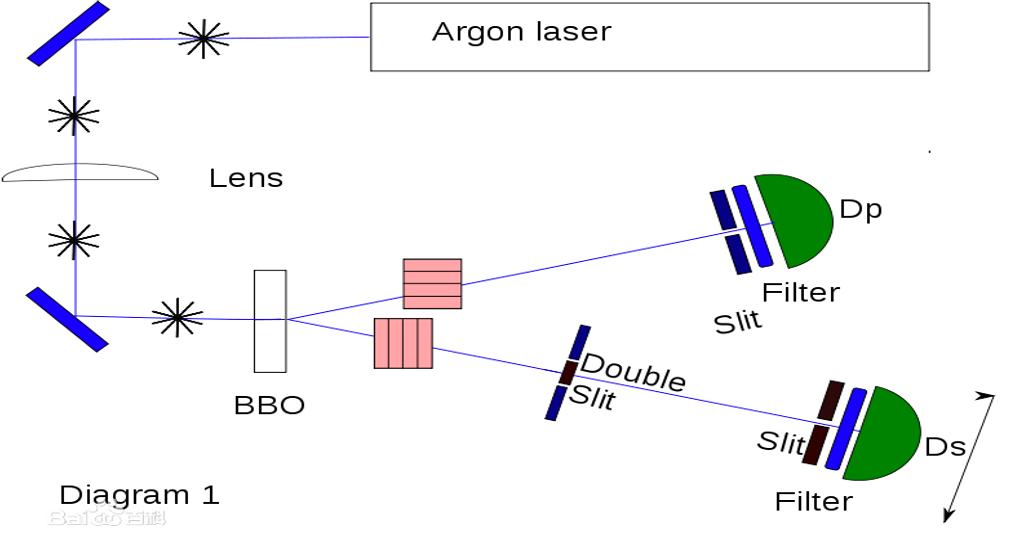
\includegraphics[width=1.0\textwidth]{figs/chachuexp.png} \\
    \end{center} 
\end{frame}

\begin{frame}
    \frametitle{}
    \begin{center}
        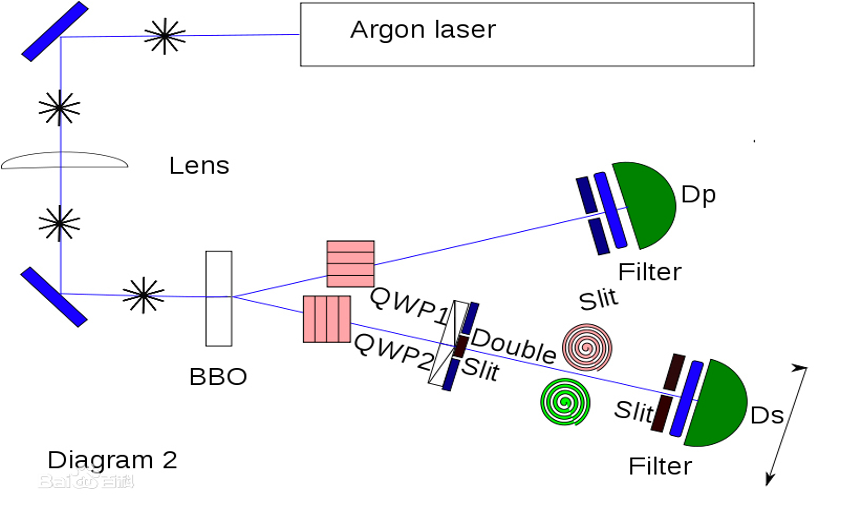
\includegraphics[width=1.0\textwidth]{figs/chachuexp_2.png} \\
    \end{center} 
\end{frame}

\begin{frame}
    \frametitle{}
    \begin{center}
        \includegraphics[width=1.0\textwidth]{figs/chachuexp_3.png} \\
    \end{center} 
\end{frame}

\begin{frame}
    \frametitle{Summary}
    \begin{enumerate}
        \item Objects are wave-particles and can be in states of superposition
        \item Measurement changes the states and gives random results
        \item Measurement results are complementary
        \item Measurement leads to objective reality
    \end{enumerate}
\end{frame}

